
%for compiling, enter
%pdflatex main_doc.tex & bibtex main_doc.aux & pdflatex main_doc.tex & pdflatex main_doc.tex

\documentclass[a4paper]{jpconf}
\bibliographystyle{iopart-num}
\usepackage{citesort}
\usepackage{amsmath}
\usepackage{booktabs}
\usepackage{color}
%% \usepackage[square,sort&compress]{natbib}

\newcommand{\REVTeX}{REV\TeX}
\newcommand{\blCom}[1]{}  %uncomment for blue comments off
%\newcommand{\blCom}[1]{\begingroup\sffamily\color{blue} #1 \endgroup}  %uncomment for blue comments on
\newcommand{\dgC}{$^\circ$C} 

\sloppy 

\usepackage{graphicx}
\begin{document}
\title{Prediction of uncertainty of 10-coefficient compressor maps for extreme operating conditions}

\author{Howard Cheung}

\address{Postdoctoral Research Fellow, Ray W. Herrick Laboratories, School of Mechanical Engineering, Purdue University, 177 S. Russell St., West Lafayette, IN 47907-2031, US}

\ead{cheung@purdue.edu}

\author{Christian K. Bach}

\address{Assistant Professor, Mechanical and Aerospace Engineering, Oklahoma State University, 218 Engineering North, Stillwater, OK 74078-5016}

\ead{cbach@okstate.edu}

\begin{abstract}
Empirical compressor maps are a simple and reliable approach for heating and cooling system designers to estimate compressor refrigerant mass flow rate and power consumption quickly. These maps were used for a long time since most compressor manufacturers build the maps with extensive test matrices, leading to good accuracy. However, the situation changes when engineers extrapolate the maps to investigate the compressor's performance under extreme operating conditions such as for cold climate heat pump applications or under conditions with system faults.  Engineers are not confident on the exact uncertainty of the extrapolation, and often claim that the inaccuracy of their studies is a result of high extrapolation uncertainty. This paper presents a method to estimate the extrapolation uncertainty due to the structure of the test matrix that trains the manufacturer maps and helps the investigators to understand if the extrapolation is the main cause of their inaccuracy. To verify that the method can estimate the uncertainty due to extrapolation, the study builds 10-coefficient compressor maps trained by different test matrices of the same size and different operating points. The maps are used to estimate the compressor performance under different operating points and their estimation uncertainties are compared. The results show that the component of the uncertainty that depends on the structure of the test matrix is small at operating conditions within the test matrix but the uncertainty grows significantly as the estimation becomes further away from the operating conditions within the test matrices.\blCom{Some comment.  See main\_doc.tex \textbackslash blCom for how to get rid of it :)}
\end{abstract}

\blCom{Introduction} %using comment to mark which subfile things come from
\section{Introduction}
\label{sec:introduction}
Empirical compressor maps for positive displacement compressors, such as the 10-coefficient polynomials outlined in ANSI/AHRI Standard 540 \cite{AHRI:540} and European Standard EN 12900 \cite{CEN:2013}  are widely used in academia and industry.  These maps are trained with experimental data and then used to calculate power input, mass flow rate, current, and compressor efficiency.  However, the maps contain squared and cubic terms of the inputs (suction and discharge dew point temperature) and are therefore potentially inaccurate when used for extrapolation outside of the training data range. Manufacturers often state an accuracy of $\pm 5 \%$ for tabulated performance data (e.g. \cite{emerson:2006} or \cite{bristol:2015}). 
This paper shows a method that estimates the resulting uncertainty for the 10 coefficient polynomial at a certain point other than the training data set. \\
This paper does not address interpolation between different speeds of variable speed compressors. However, the shown methodology can be extended to predict the uncertainty of the outputs for interpolating between fixed speeds rather than using different fixed speed compressor maps as done by e.g.  \cite{shen:2014} and \cite{caskey:2012}.

\blCom{Linear\_regression}
\section{Linear regression}
\label{sec:linear_regression}
Finding the coefficients of the 10 coefficient maps can be treated as a linear regression problem, with the evaporation and condensing temperature and their linear, squared and cubed combinations being the independent variables ${\vec x}$ and the power consumption of the compressor being the estimated dependent variable $y$. To better understand the uncertainty sources of the model, a brief review of linear regression along with how this applies to the polynomial compressor map is shown subsequently.

\subsection{Review}
\label{sec:linreg_review}
Linear regression is used to estimate the parameters of a linear model.  Measurement data always includes error, therefore only an estimate of the true parameters can be obtained. If we had the true model parameters ${\vec \beta _{true}} $, then we could use the independent inputs to our model (${\vec x^T}$) to calculate the true output $y_{true}$ up to an error $\varepsilon$ caused by measurement error \blCom{The $\varepsilon$ is not caused by measurement error, but the inability of a linear model to describe the inifinte number of output variables $y$ within the operating range},

\begin{equation}
{y_{true}} = {\vec x^T}{\vec \beta _{true}} + \varepsilon .
\label{eq:true_lin_model}
\end{equation}

Unfortunately it is not possible to obtain the true model, since all measurement data that is used for training the model includes measurement error \blCom{No. The true model is impossible to obtain because it is impossible to obtain the infinite number of data points within the operating range.}. Therefore, we need to estimate the model parameters to be able to calculate an estimate of the output. To emphasize the difference between the two models, a hat ( $\hat{}$ ) is used for both, estimated model parameters $\hat {\vec \beta}$ and estimated model output, $\hat y$,

\begin{equation}
\hat y = {\vec x^T}\hat {\vec \beta}.
\label{eq:estimted_lin_model}
\end{equation}

The parameters for the model can be estimated using measurement data, for non-weighted reduction of the squares of the errors it can be shown that the  parameter vector $\hat {\vec \beta}$ can be calculated as

\begin{equation}
\hat {\vec \beta}  = {({\mathbf{X}}_{train}^T{{\mathbf{X}}_{train}})^{ - 1}}{\mathbf{X}}_{train}^T{\vec y_{train}},
\label{eq:estimte_parameters}
\end{equation}

where the subscript $train$ is used for training data, the training data input matrix ${{\mathbf{X}}_{train}}$, composed of input data vectors ${\vec x}_{train,i}$ for each data point $i$ is constructed as

\begin{equation}
 {{\mathbf{X}}_{train}} = {\left[ {\begin{array}{*{20}{c}} {{{\vec x}_{train,1}}}& \cdots &{{{\vec x}_{train,i}}}& \cdots &{{{\vec x}_{train,n}}}
\end{array}} \right]^T},
\label{eq:input_tr_matrix}
\end{equation}

where $n$ is the total number of data points. The output training data vector is composed of output values $y_{train,i}$ for each data point as

\begin{equation}
{\vec y_{train}} = {\left[ {\begin{array}{*{20}{c}}
  {{y_{train,1}}}& \cdots &{{y_{train,i}}}& \cdots &{{y_{train,n}}} 
\end{array}} \right]^T}.
\label{eq:output_tr_vector}
\end{equation}

The accuracy of the model, measured by the mean sum of square $\sigma$, is 

\begin{equation}
\sigma  = \sqrt {\frac {{\Sigma _i}{{({y_{train,i}} - {{\vec x}^T}\hat {\vec \beta} )}^2}} {n - 1}}.
\label{eq:acc_est_model}
\end{equation}

\subsection{Polynomial compressor map as linear regression problem}
\label{sec:linreg_compmap}
ANSI/AHRI Standard 540 \cite{AHRI:540} estimates the compressor power consumption $\hat {\dot W}$ as

\begin{equation}
\begin{gathered}
  \hat {\dot W} = {\beta _1} + {\beta _2}{T_{evap}} + {\beta _3}{T_{cond}} + {\beta _4}T_{evap}^2 + {\beta _5}{T_{evap}}{T_{cond}} + {\beta _6}T_{cond}^2 + {\beta _7}T_{evap}^3 + \\
  {\beta _8}T_{evap}^2{T_{cond}} + {\beta _9}{T_{evap}}T_{cond}^2   + {\beta _{10}}T_{cond}^3 ,
\end{gathered} 
\label{eq:pwr_map_definition}
\end{equation}

where $\beta_i$ are the (estimated) model coefficients and $T_{evap}$, and $T_{cond}$ are the evaporation and condensing dew point temperatures. Referring to eqn. \ref{eq:estimted_lin_model}, $\hat {\dot W}$ takes the place of $\hat y$, the estimated parameter vector  $\hat {\vec \beta}$ is composed of the $\beta_i$, and the vector of independent variables (here: dew point temperatures), $\vec x$ is constructed as

\begin{equation}
\begin{split}
&\vec x = \\
&{\left[ {\begin{array}{*{20}{c}}
  1&{{T_{evap}}}&{{T_{cond}}}&{T_{evap}^2}&{{T_{evap}}{T_{cond}}}&{T_{cond}^2}&{T_{evap}^3}&{T_{evap}^2{T_{cond}}}&{\begin{array}{*{20}{c}}
  {{T_{evap}}{T_{cond}}}&{T_{cond}^3} .
\end{array}} 
\end{array}} \right]^T}
\end{split}
\label{eq:lin_reg_temp_vec}
\end{equation}


\blCom{unc\_steady}
\section{Uncertainty of steady state measurements}
\label{sec:unc_steady}
The training data for compressor maps is obtained from steady state time series data. Steady state time series data do not show any significant monotonic trends with time but rather shows periodic and random fluctuations (noise) around an average value. The mean value $a$ of the measured variable can be defined as

\begin{equation}
a = \Sigma _{i = 1}^N{\frac{{{a_{mea}}({t_i})}}{N}},
\label{eq:avg_mea}
\end{equation}

where $a_{mea}(t_i)$ is a discrete measurement of the variable at time step $i$, and $N$ is the number of measurements in a time serires. Measurement devices have a time-independent uncertainty often called zero-order uncertainty. The limited number of samples in combination with the fluctuations of the variable due to environmental noise leads to the first-order uncertainty.  Zero-order uncertainty is typically provided by the manufacturer of the measurement device, such as $\pm0.5K$ for T-type thermocouples, or $0.5\%$ of the measured flow rate for Coriolis mass flow meters. First-order uncertainty is not known in advance but rather needs to be approximated by statistically analyzing the time series data of the steady state measurement. Taylor and Kuyatt (1994)\cite{Kamei:1995} give the overall measurement uncertainty as

\begin{equation}
\Delta a = \sqrt {\Sigma _{i = 1}^N{{\left(\frac{{\Delta {a_{mea}}({t_i})}}{N}\right)}^2} + {{\left(\frac{{{t_{N - 1,1 - \alpha /2}}}}{N}\right)}^2}\frac{{\Sigma _{i = 1}^N{{\left({a_{mea}}({t_i}) - a\right)}^2}}}{{N - 1}}} 
\label{eq:mea_unc_TK}
\end{equation}

where $t_{N-1,1-\alpha/2}$ is the statistic of the Student's \emph{t}-distribution with a degree of freedom of N-1 and level at $1-\alpha/2$. The first part of the uncertainty is the sum of squares of the zero-order uncertainty of each observation within the steady state measurement. The second part of the uncertainty is given as the confidence interval of the average value at the level of $1-\alpha/2$. In practice, $\alpha$ is taken as 0.1, and a 95\% confidence interval is usually used in the approximation.

\blCom{Approx\_uncertainty}
\section{Generating experimental results of steady state data with uncertainties from compressor map data}
\label{sec:approx_uncertainty}
For this paper, no real measurement data are taken for training data, and only ideal compressor performance data from the manufacturers without uncertainty is available. In order to test the uncertainty calculation of the compressor map output, some training data is needed. Hence it is necessary to approximate a set of training data with uncertainties from the ideal compressor performance data. If the ideal compressor performance data are the true values of the measurement, its measurement value will be different from its true value because it is subjected to the zero-order uncertainty of the measurement device and the first-order uncertainty of the noise of the measurement environment.  Assuming that the uncertainty is the confidence interval of the measurement value at a level of $1-\alpha/2$ and the measurement value follows a normal distribution with a mean value around the true value of the measurement, the standard deviation of the normal distribution will be given by

\begin{equation}
{\sigma _{mea}} = \frac{{\sqrt {{{(\Delta {a_{zero - order}}(a = {a_{true}}))}^2} + {{(\Delta {a_{first - order}}(a = {a_{true}}))}^2}} }}{{{z_{1 - \alpha /2}}}}
\label{eq:std_norm}
\end{equation}

where $z_{1-\alpha/2}$ is the z-normal distribution statistics given at a level of ${1-\alpha/2}$. The observations within steady state can then be approximated by running a random number generator following a normal distribution with mean at the true value of a and standard deviation at σmea multiple times. These values can then be analyzed with the method listed in the section~\ref{sec:unc_steady} to calculate the value and uncertainty of steady state measurement.

\blCom{sources\_of\_uncertainty}
\section{Sources of uncertainty} \label{sec:sources}
\label{sec:uncer_source}

Uncertainty of the compressor map output is the range where the true value of the output may be relative to the map output. It consists of multiple components and can be grouped as follows:

\begin{itemize}
\item Uncertainty due to inputs
\item Uncertainty due to training data
\item Uncertainty due ot model random error
\item Uncertainty due to outputs
\end{itemize}

\subsection{Uncertainty due to inputs} \label{subsec:uncer_inputs}
Uncertainty due to inputs is the uncertainty propagated to the map output due to the uncertainty in the inputs to the maps. The inputs to the map (evaporating and condenser temperature) are usually obtained by converting pressure measurements to saturation temperatures with refrigerant equations of state. Therefore the estimated saturation temperature contains uncertainty from both the equation of state and the pressure measurement. The equation of state of R22 estimates saturation pressure at an uncertainty of 0.2\% \cite{Kamei:1995}. When the equation of state estimates an saturation temperature at a given pressure, this uncertainty is transformed into a component of the uncertainty of the saturation temperature as shown in

\begin{equation}
\frac{\Delta P_{sat,EOS}}{P_{sat}(T)} = 0.2\% = 0.002
\label{eq:uncer_p_eos}
\end{equation}

and

\begin{equation}
\Delta {T_{sat,EOS}} = \left|{\frac{{\partial {T_{sat}}({P})}}{{\partial {P}}}}\right|\Delta {P_{sat,EOS}} ,
\label{eq:uncer_t_eos}
\end{equation}

where $\Delta P_{sat,EOS}$ is the uncertainty of saturation pressure as a result of uncertainty of the equation of state, $P_{sat}(T)$ is the saturation pressure from temperature $T$, $\Delta {T_{sat,EOS}}$ is the uncertainty of saturation temperature as a result of uncertainty of the equation of state and ${T_{sat}}({P})$ is the saturation temperature at pressure $P$.

The component of the saturation temperature uncertainty due to pressure measurement is calculated by

\begin{equation}
\Delta {T_{sat,mea}} = \left|\frac{{\partial {T_{sat}}({P})}}{{\partial {P}}}\right|\Delta {P_{sat,mea}},
\label{eq:uncer_t_mea}
\end{equation}

where $\Delta {T_{sat,mea}}$ is the uncertainty of saturation temperature as a result of pressure measurement and $\Delta P_{sat,mea}$ is the uncertainty of pressure measurement. The overall uncertainty of the saturation temperature is given by 

\begin{equation}
\Delta {T_{sat}} = \sqrt {{{(\Delta {T_{sat,EOS}})}^2} + {{(\Delta {T_{sat,mea}})}^2}} .
\label{eq:uncer_t}
\end{equation}

The uncertainty of the map output propagated from the inputs of condensing temperature and evaporating temperature is calculated by

\begin{equation}
\Delta {\hat{\dot{W}}_{input}} = \sqrt {{\left(\frac{{\partial \hat{\dot{W}}}}{{\partial {T_{evap}}}}\Delta {T_{evap}}\right)^2} + {\left(\frac{{\partial \hat{\dot{W}}}}{{\partial {T_{cond}}}}\Delta {T_{cond}}\right)^2}}, 
\label{eq:uncer_w_input}
\end{equation}

where $\Delta {\hat{\dot{W}}_{input}}$ is the uncertainty due to inputs at the map output, $\Delta {T_{evap}}$ is the uncertainty of evaporating temperature at input and $\Delta T_{cond}$ is the uncertainty of condensing temperature at input

\subsection{Uncertainty due to training data} \label{subsec:uncer_train}
Uncertainty due to training data is the uncertainty propagated to the map output from the training data through the map coefficients. This can be understood by considering the estimation of the map coefficients as a function of the training data as

\begin{equation}
\hat{ \vec {\beta}}  = g({T_{evap,train,1}},...,{T_{evap,train,n}},{T_{cond,train,1}},...,{T_{cond,train,n}},{\dot{W}_{train,1}},...,{\dot{W}_{train,n}}), 
\label{eq:beta_train}
\end{equation}

where n is the number of training data points. Through function $g$ and $\hat{ \vec {\beta}}$ in Eqn. (\ref{eq:beta_train}), as suggested in \cite{song:2013}, the uncertainty component due to training data is calculated

\begin{equation}
\Delta {\hat{\dot{W}}_{train}} = \sqrt{\begin{gathered}
  \Sigma_{j=1}^n\left(\Sigma _{i = 1}^m\left(\frac{{\partial \hat{\dot{W}}}}{{\partial {\beta _i}}}\frac{{\partial {\beta _i}}}{{\partial {T_{evap,train,j}}}}\right)\Delta {T_{evap,train,j}}\right)^2  \hfill \\
  +\Sigma_{j=1}^n\left(\Sigma _{i = 1}^m\left(\frac{{\partial \hat{\dot{W}}}}{{\partial {\beta _i}}}\frac{{\partial {\beta _i}}}{{\partial {T_{cond,train,j}}}}\right)\Delta {T_{cond,train,j}}\right)^2 \hfill \\
   +\Sigma_{j=1}^n\left(\Sigma _{i = 1}^m\left(\frac{{\partial \hat{\dot{W}}}}{{\partial {\beta _i}}}\frac{{\partial {\beta _i}}}{{\partial {\dot{W}_{,train,j}}}}\right)\Delta {\dot{W}_{train,j}}\right)^2 \hfill \\ 
\end{gathered}}, 
\label{eq:uncer_w_train}
\end{equation}

where $\Delta {\hat{\dot{W}}_{train}}$ is the uncertainty due to training data at the map output, $\Delta {T_{evap,train,j}}$ is the uncertainty of the evaporating temperature at the j$^{th}$ data point, $\Delta {T_{cond,train,j}}$ is the uncertainty of the condensing temperature at the j$^{th}$ data point, $\Delta {\dot{W}_{train,j}}$ is the uncertainty of the power consumption at the j$^{th}$ data point, and m is the number of coefficients in $\hat{\vec{\beta}}$.

\subsection{Uncertainty due to model random error} \label{subsec:uncer_model}

In linear regression, the random error between true model and actual system, $\varepsilon$ in Eqn. (\ref{eq:true_lin_model}) is assumed to be normally distributed around zero with some finite variance. This variance becomes part of the uncertainty of the uncertainty of the map output and can be presented in the form of confidence intervals. Statistic textbooks \cite{Montgomery:2005,Graybill:1994} illustrated that the confidence interval of the variance can be calculated as

\begin{equation}
\Delta {\hat{\dot{W}}_{model}} = {t_{n - m,1 - \alpha /2}}\sigma \sqrt {1 + {{\vec x}^T}{{({\mathbf{X}}_{train}^T{{\mathbf{X}}_{train}})}^{ - 1}}\vec x}
\label{eq:uncer_w_model}
\end{equation}

where $\Delta {\hat{\dot{W}}_{train}}$ is the uncertainty due to model random error at the map output.

One significant term in Eqn. (\ref{eq:uncer_w_model}) is ${\vec x^T}{({\mathbf{X}}_{train}^T{{\mathbf{X}}_{train}})^{ - 1}}\vec x$ which is the leverage of a regression model \cite{Atkinson:1987}. It estimates how deviated the current input vector to the map is relative to the training data of the regression model, and the magnitude of the leverage grows with the deviation. This helps to understand if the estimation is related to the training data and if (or ``how much'')the model is applicable at the current situation described by the input vector.

\subsection{Uncertainty due to output} \label{subsec:uncer_output}

Uncertainty of the map output should represent the probable range where the true value lies relative to the map output. However, since the map is built from data obtained from measured power consumption instead of true values of the power consumption, the uncertainty components of the map output propagated from other sources only estimate the uncertainty of the estimation with the measured power consumption. Another component of uncertainty must be introduced so that the map output uncertainty is the uncertainty to the true map output. This uncertainty component can be approximated with the uncertainty of the measured power consumption with its true values by

\begin{equation}
\Delta {\hat{\dot{W}}_{output}} = \frac{1}{n}\Sigma _{i = 1}^n\frac{{\Delta {{\dot{W}}_{train,i}}}}{{{{\dot{W}}_{train,i}}}} .
\label{eq:uncer_w_output}
\end{equation}

\subsection{Overall uncertainty} \label{subsec:overall_uncer}

The overall uncertainty of the map output is given by the square of the sum of all uncertainty components as

\begin{equation}
\Delta \hat{\dot{W}}= \sqrt {{{(\Delta {{\hat{\dot{W}}}_{input}})}^2} + {{(\Delta {{\hat{\dot{W}}}_{train}})}^2} + {{(\Delta {{\hat{\dot{W}}}_{model}})}^2} + {{(\Delta {{\hat{\dot{W}}}_{output}})}^2}} .
\label{eq:overall_uncer}
\end{equation}

\blCom{Results\_Discussion\_CB}
\input{Results_Discussion_CB}


\blCom{comp\_map\_uncen}
\subsection{Effect of range of training data on map output} \label{subsec:comp_uncer}

To study how the range of training data affects the extrapolation uncertainty and accuracy, the difference between the map output and approximated measurement and the map output uncertainty for all data points in Figure \ref{fig:oper_envelope} are plotted in Figure \ref{fig:rel_uncer}, and a similar figure with their uncertainty components is plotted in Figure \ref{fig:uncer_comp}.

\begin{figure}[h]
\begin{minipage}{15pc}
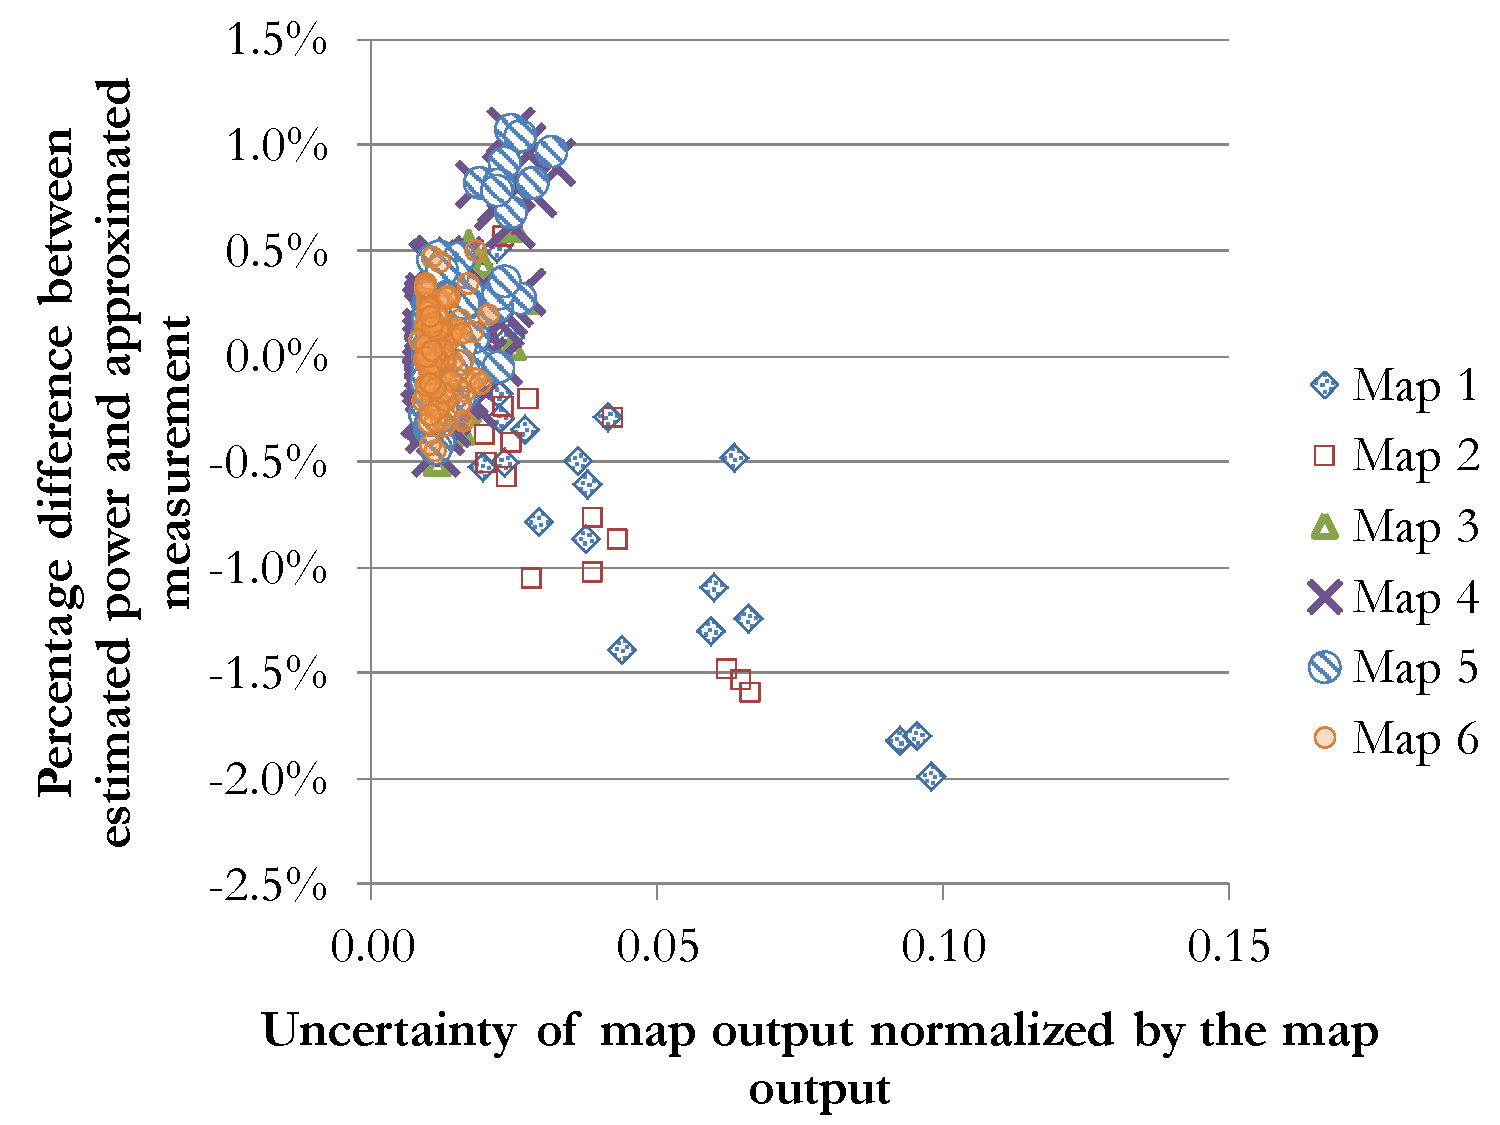
\includegraphics[width=15pc]{rel_diff_to_rel_uncer.pdf}
\caption{\label{fig:rel_uncer}Change of accuracy of maps with output uncertainty in different maps.}
\end{minipage}\hspace{2pc}%
\begin{minipage}{15pc}
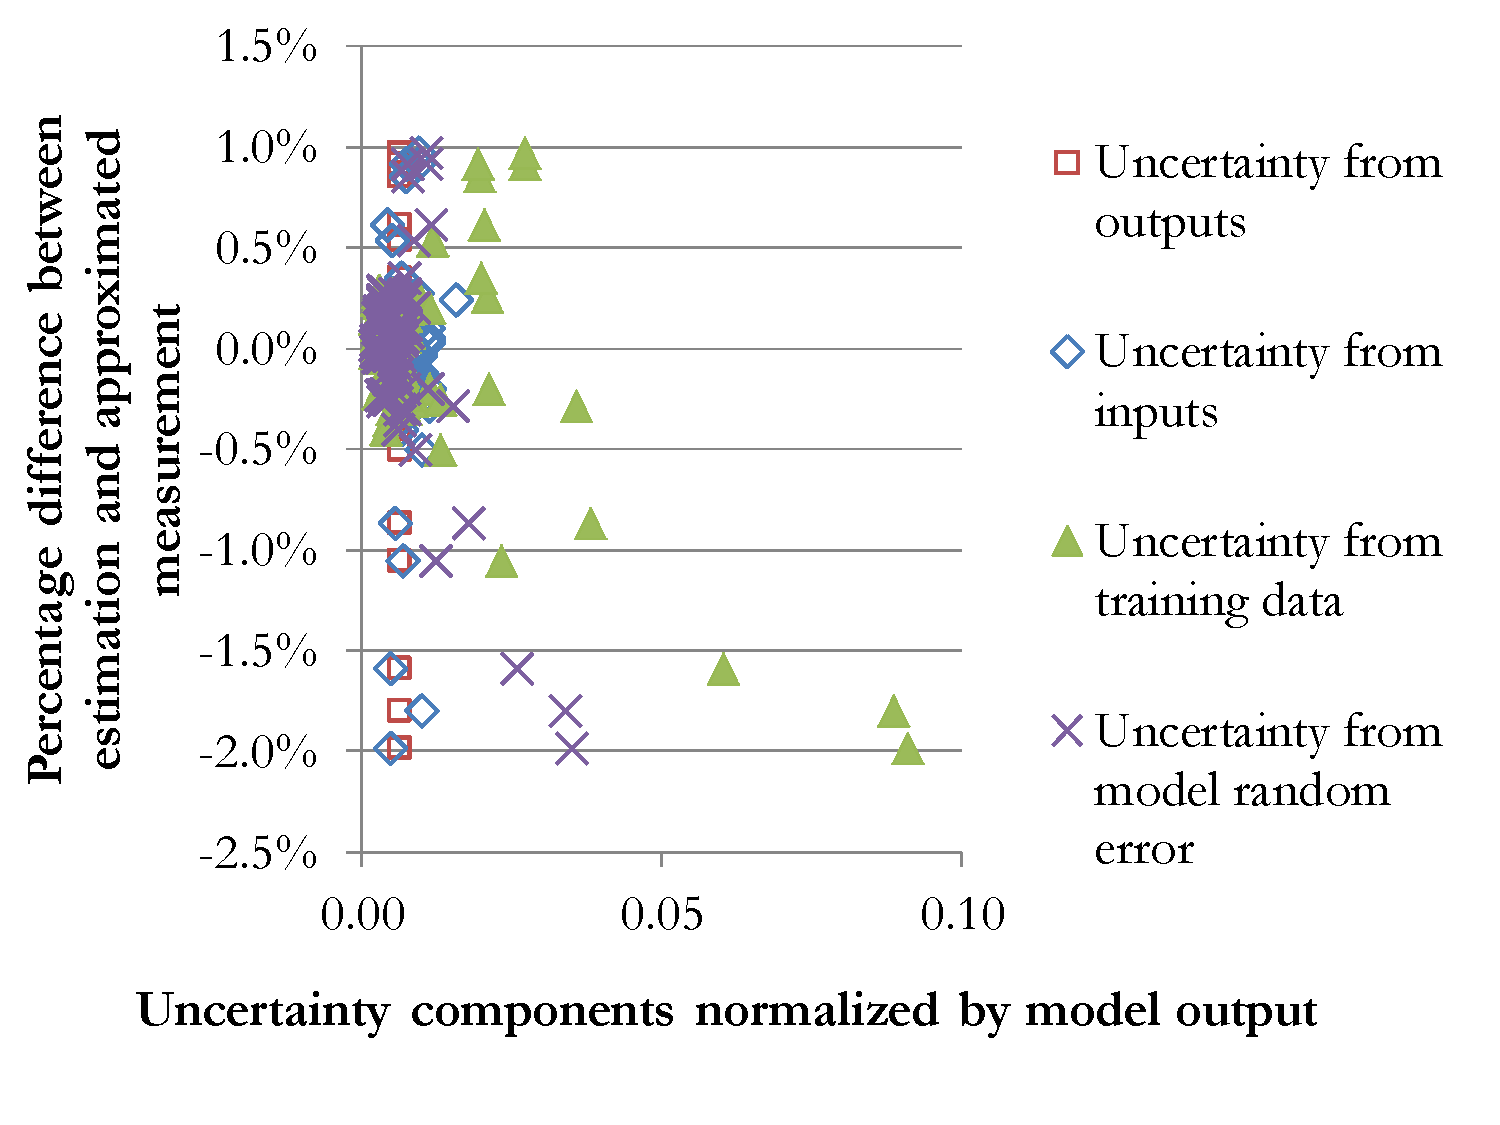
\includegraphics[width=15pc]{rel_diff_to_uncer_comp.pdf}
\caption{\label{fig:uncer_comp}Change of accuracy of maps with different uncertainty components.}
\end{minipage} 
\end{figure}

Figure \ref{fig:rel_uncer} shows that inaccurate map outputs are associated with higher uncertainty and the uncertainty calculation method is a good indicator of the accuracy of the map output. Figure \ref{fig:uncer_comp} shows that the high uncertainty of the inaccurate data points in Figure \ref{fig:rel_uncer} are primarily a result of high uncertainty from model random error and training data.

The increase of uncertainty from model random error with inaccuracy can be explained by the leverage term ${\vec x^T}{({\mathbf{X}}_{train}^T{{\mathbf{X}}_{train}})^{ - 1}}\vec x$ in Eqn. (\ref{eq:uncer_w_model}) which increases as the map extrapolates, and map extrapolation results in lower accuracy. Hence the uncertainty from model random error increase with a decrease of the map accuracy and applicability.

To explain the increase of uncertainty from training data with a decrease of map accuracy in Figure \ref{fig:uncer_comp}, the squared terms in Eqn. (\ref{eq:uncer_w_train}) are labeled as uncertainty from training data per measurement, and their values from two map outputs of Map 1 are plotted as Figures \ref{fig:map_1_low_uncer} and \ref{fig:map_1_high_uncer}.

\begin{figure}[h]
\begin{minipage}{15pc}
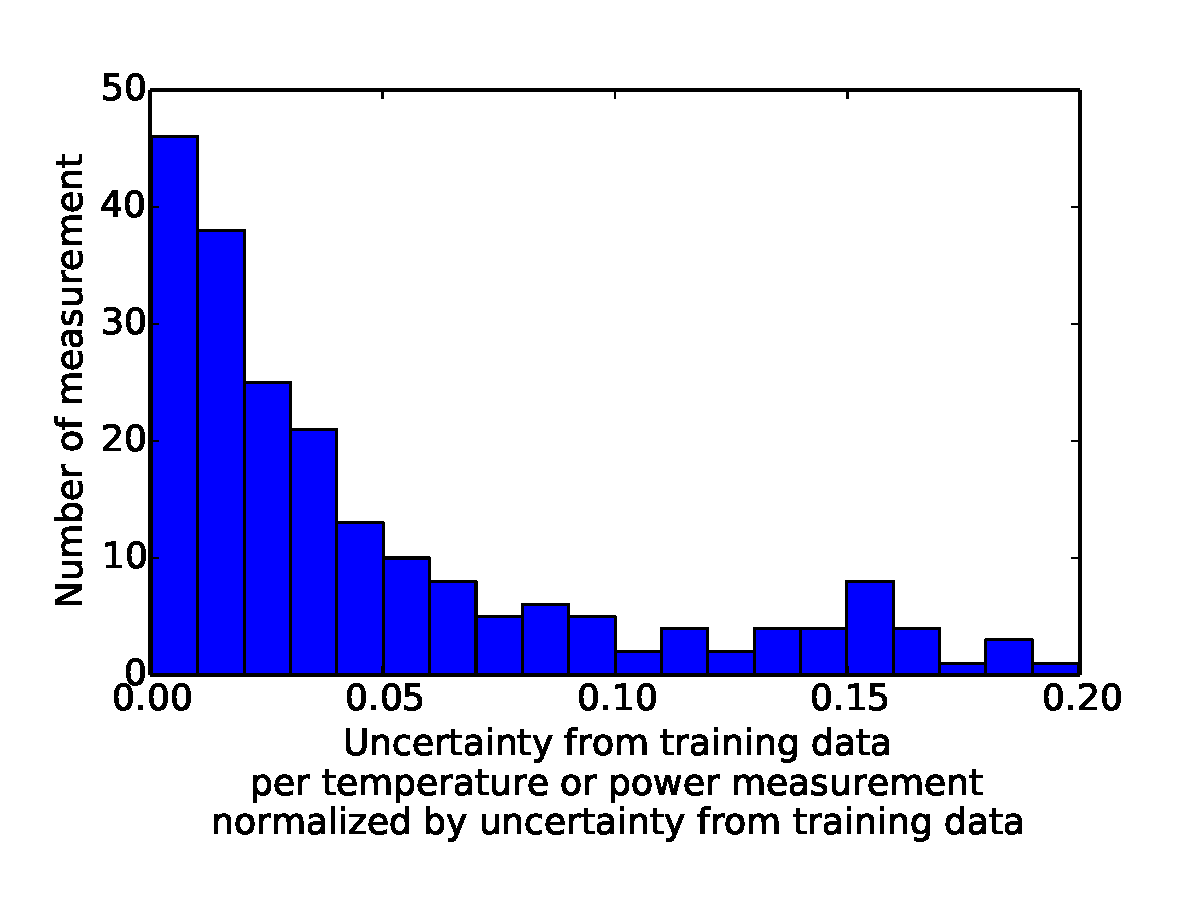
\includegraphics[width=15pc]{Map_1_low_uncer.pdf}
\caption{\label{fig:map_1_low_uncer}Histogram of uncertainty terms in Eqn. (\ref{eq:uncer_w_train}) for $T_{evap} = -1.1^\circ C$ and $T_{cond} = 60.0^\circ C$.}
\end{minipage}\hspace{2pc}%
\begin{minipage}{15pc}
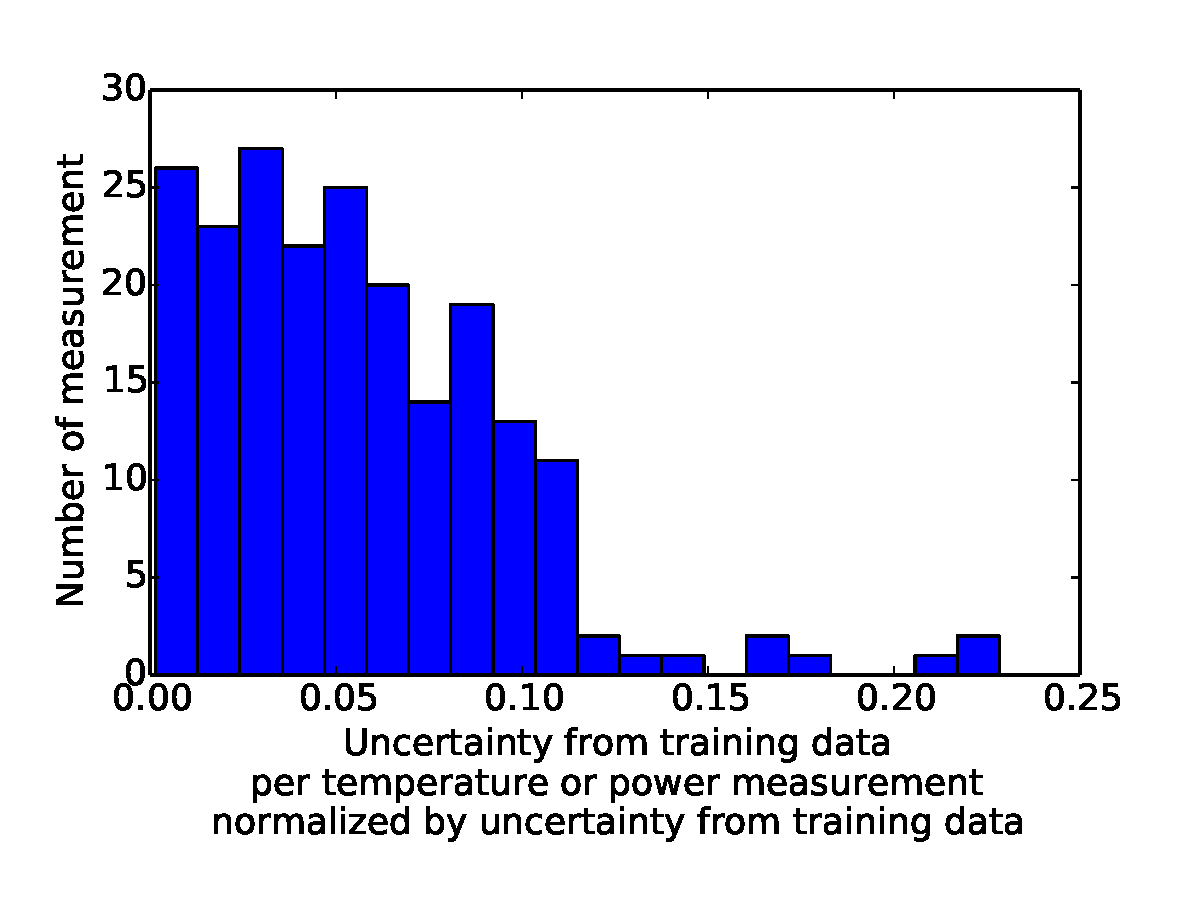
\includegraphics[width=15pc]{Map_1_high_uncer.pdf}
\caption{\label{fig:map_1_high_uncer}Histogram of uncertainty terms in Eqn. (\ref{eq:uncer_w_train}) for $T_{evap} = -28.9^\circ C$ and $T_{cond} = 26.7^\circ C$.}
\end{minipage} 
\end{figure}

Figure \ref{fig:map_1_low_uncer} shows a histogram that is more left-skewed than Figure \ref{fig:map_1_high_uncer}. This is because Figure \ref{fig:map_1_low_uncer} is obtained from a data point inside the training data range of Map 1 (see Figure~\ref{fig:training_envelope}), and the map only needs information from a few data points around $T_{evap} = -1.1^\circ C$ and $T_{cond} = 60.0^\circ C$ to estimate its map output. Hence the estimation does not depend on most of the data points, and their training data uncertainties do not propagate to the map output as shown by Figure \ref{fig:map_1_low_uncer}. 

However, Map 1 extrapolates to the lower left handed corner in Figure \ref{fig:training_envelope} for the condition in Figure \ref{fig:map_1_high_uncer}, and the estimation is significantly affected by multiple data points in the training data. If any of these significant training data points change, the estimation result at this condition will be changed significantly. Hence much more training data points propagate their uncertainty to the map output under the condition in Figure \ref{fig:map_1_high_uncer} than that in Figure \ref{fig:map_1_low_uncer}. This also explains that the uncertainty of training data is a significant component in the extrapolation uncertainty of the map output, and the uncertainty increases as the map applicability and accuracy decrease.


\blCom{num\_train}
\subsection{Effect of number of training data points on map output} \label{subsec:num_train}

To understand how the number of training data points affect the map output, another map (Map 7) was created with the same range of training data as Map 1 and 24 data points only, as shown in Figure \ref{fig:map_1_7_training_data}. The accuracy of Map 7, rated by coefficient of variation $cov$ as 

\begin{equation}
cov = \frac{\text{Sum of squares of errors}}{\text{Mean value of estimated values}} = \frac{\text{Sample standard deviation}}{\text{Mean value of estimated values}} = \frac{\sigma}{1/n\cdot\Sigma_1^n \hat{y}_i}
\label{eq:cov}
\end{equation}
\blCom{changed above formula, please double-check if correct}
is compared with that of Map 1 in Table \ref{tb:map7_acc}.

\begin{table}[h]
\caption{\label{tb:map7_acc}Accuracy of Maps 1 and 7.}
\begin{center}
\begin{tabular}{p{1.2cm} p{6cm} p{5.7cm}}
\br
Map & Coefficient of variation based on training data poinst only ($cov_{train}$) & Coefficient of variation based on all data points in Figure \ref{fig:oper_envelope} ($cov_{all}$) \\
\mr
Map 1&0.18\%&0.31\%\\
Map 7&0.17\%&1.10\%\\
\br
\end{tabular}
\end{center}
\end{table}

Table \ref{tb:map7_acc} shows that the accuracy of Map 7 is similar to that of Map 1 at the training data points, but the analysis with all available data points shows that Map 7 is less accurate than Map 1. This shows that using fewer training data points reduces map accuracy. But to know if the reduction of accuracy happens at extrapolation, the accuracy of the map outputs is compared with the uncertainty from model random error and the uncertainty from training data as shown in Figures \ref{fig:num_train_model} and \ref{fig:num_train_train}.

\begin{figure}[h]
\begin{minipage}{15pc}
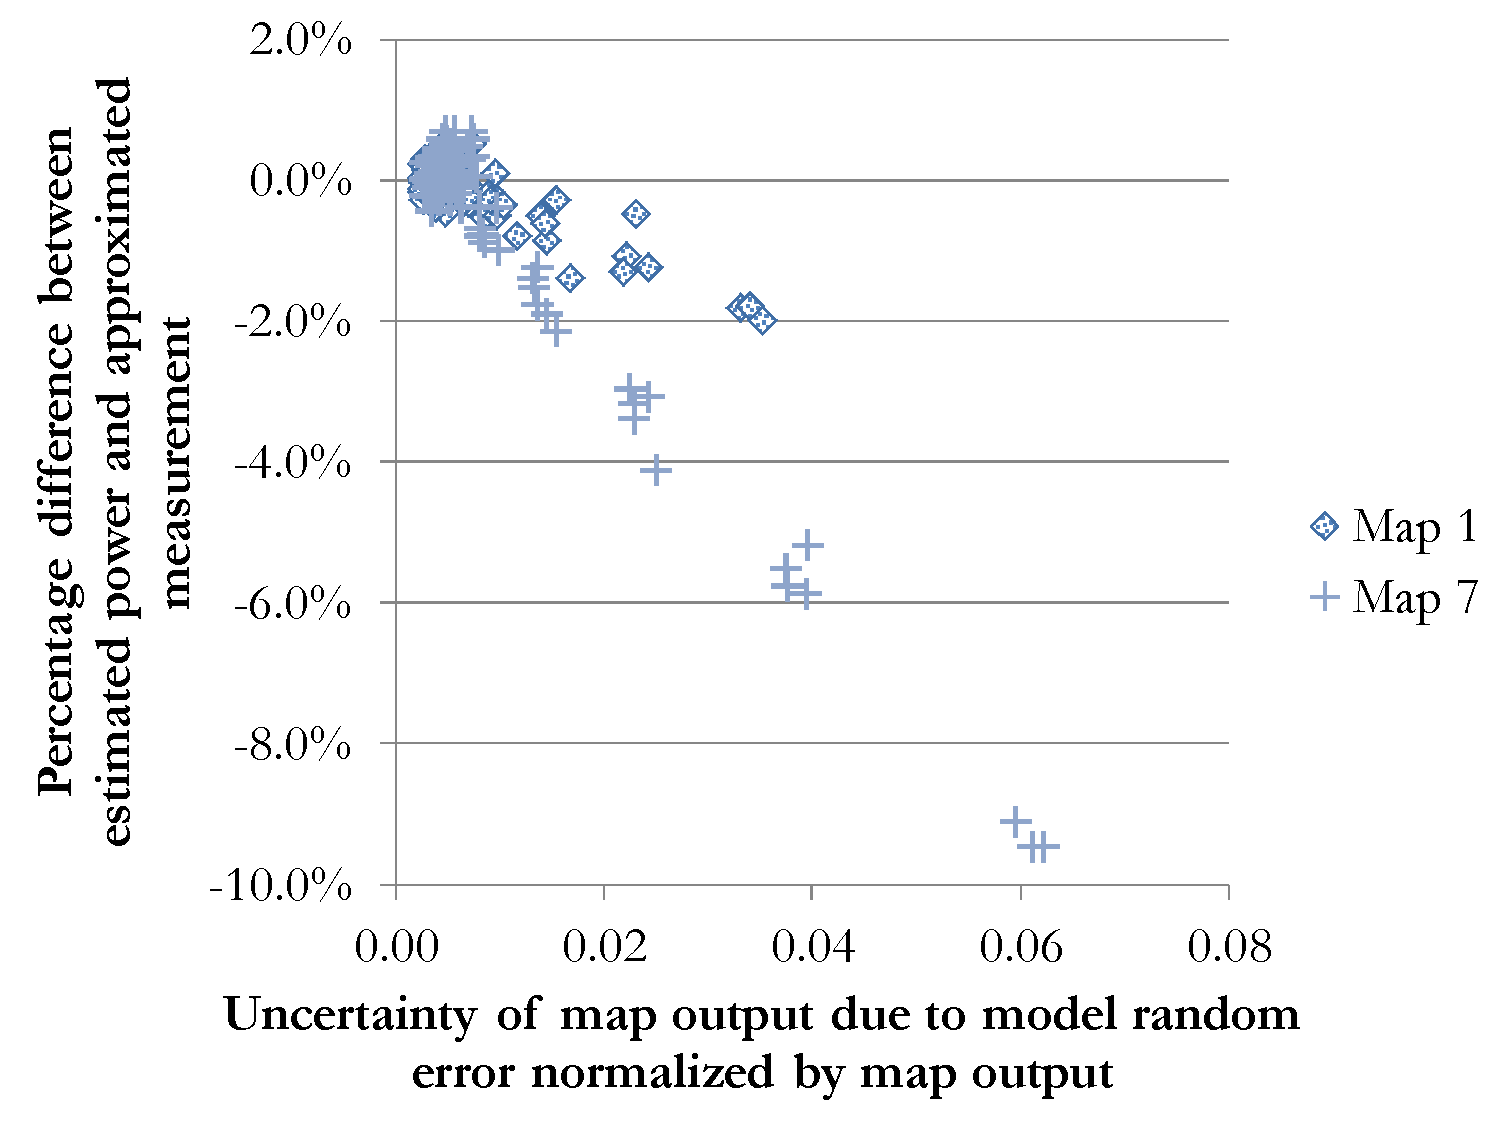
\includegraphics[width=15pc]{num_train_model.pdf}
\caption{\label{fig:num_train_model}Change of accuracy of maps with uncertainty from model random error in Maps 1 and 7.}
\end{minipage}\hspace{2pc}%
\begin{minipage}{15pc}
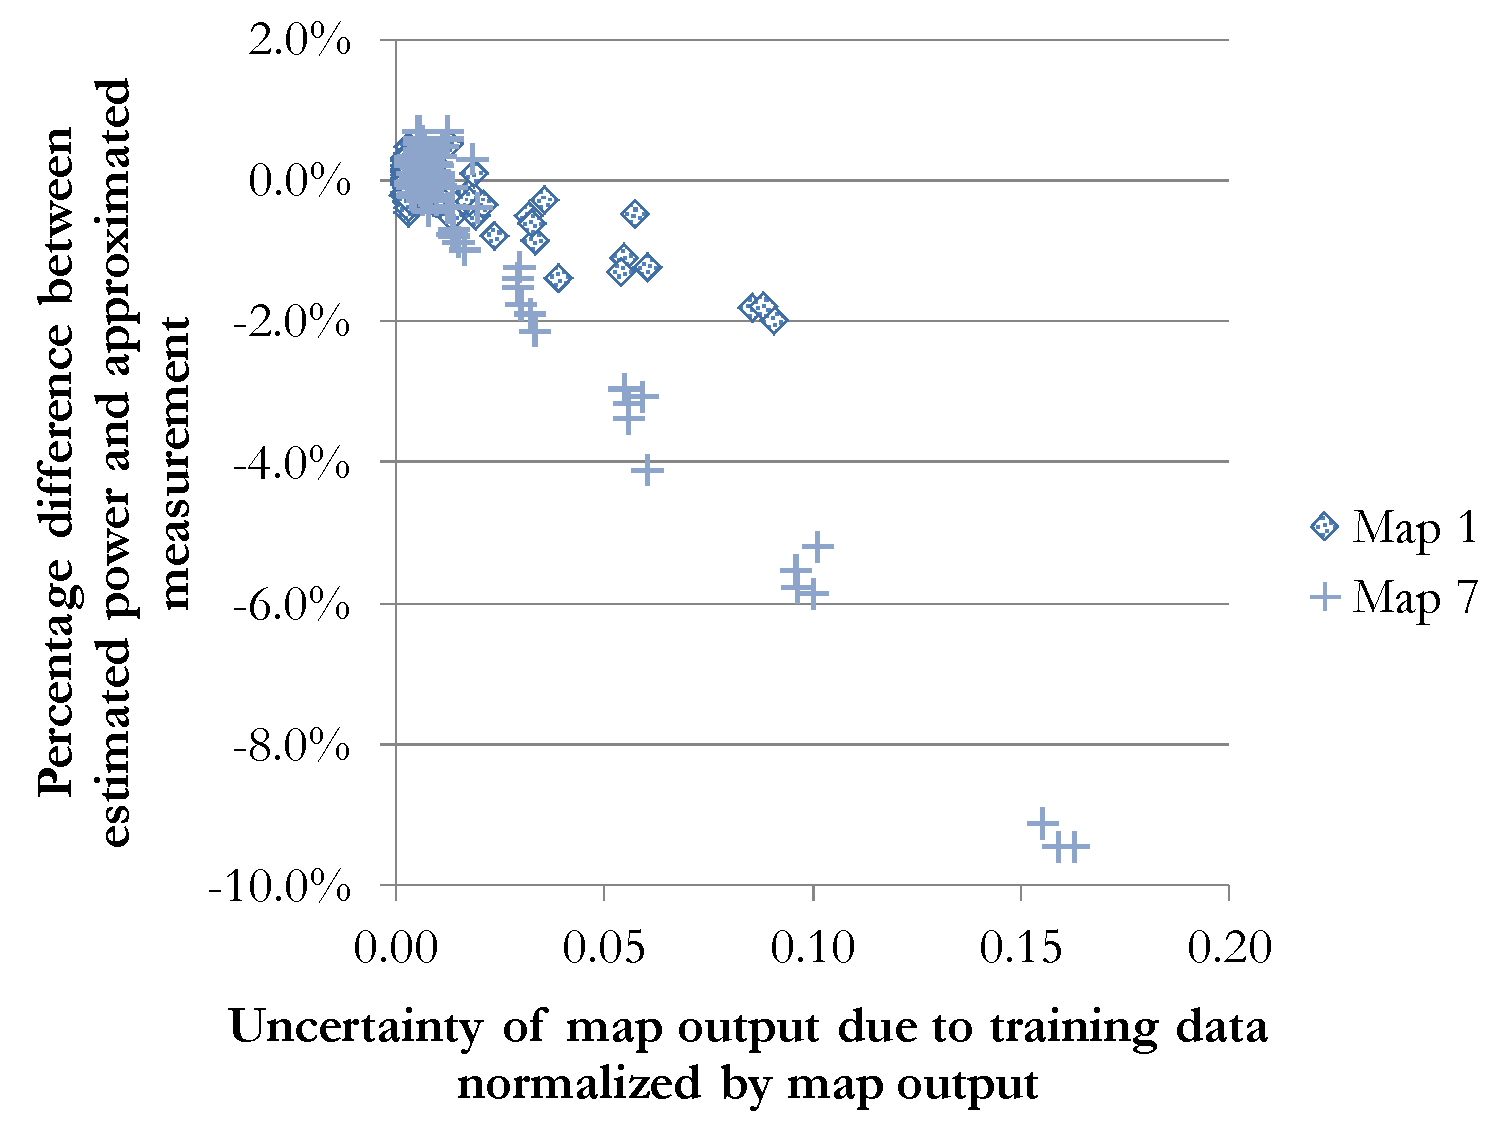
\includegraphics[width=15pc]{num_train_train.pdf}
\caption{\label{fig:num_train_train}Change of accuracy of maps with uncertainty from training data in Maps 1 and 7.}
\end{minipage} 
\end{figure}

Figures \ref{fig:num_train_model} and \ref{fig:num_train_train} show that both the accuracy of Maps 1 and 7 decreases as their uncertainty from model random error and the uncertainty from training data increase, and the reduction of Map 1 accuracy in both figures are more rapid than Map 7. This shows that Map 7, despite having the same training data range as Map 1, is less applicable and accurate as Map 1. This shows that extrapolation uncertainty and accuracy are not only affected by the range of training data but also the number of training data points.\\

The effect of the reduced number of points in the training data is a larger uncertainty for the same distance, e.g. $\sqrt{\Delta T_{cond}^2 + \Delta T_{evap}^2}$, from the nearest training data point as shown in Figure~\ref{fig:map_1_7_unc_C_distance}.  This effect is especially pronounced for large distances (e.g. extrapolated outside training data range of map) of 10\dgC{} or larger and can increase the uncertainty from 10\% (Map 1) to approximately 17\% (Map 7) in the most extreme case.

\begin{figure}[h]
\begin{minipage}{15pc}
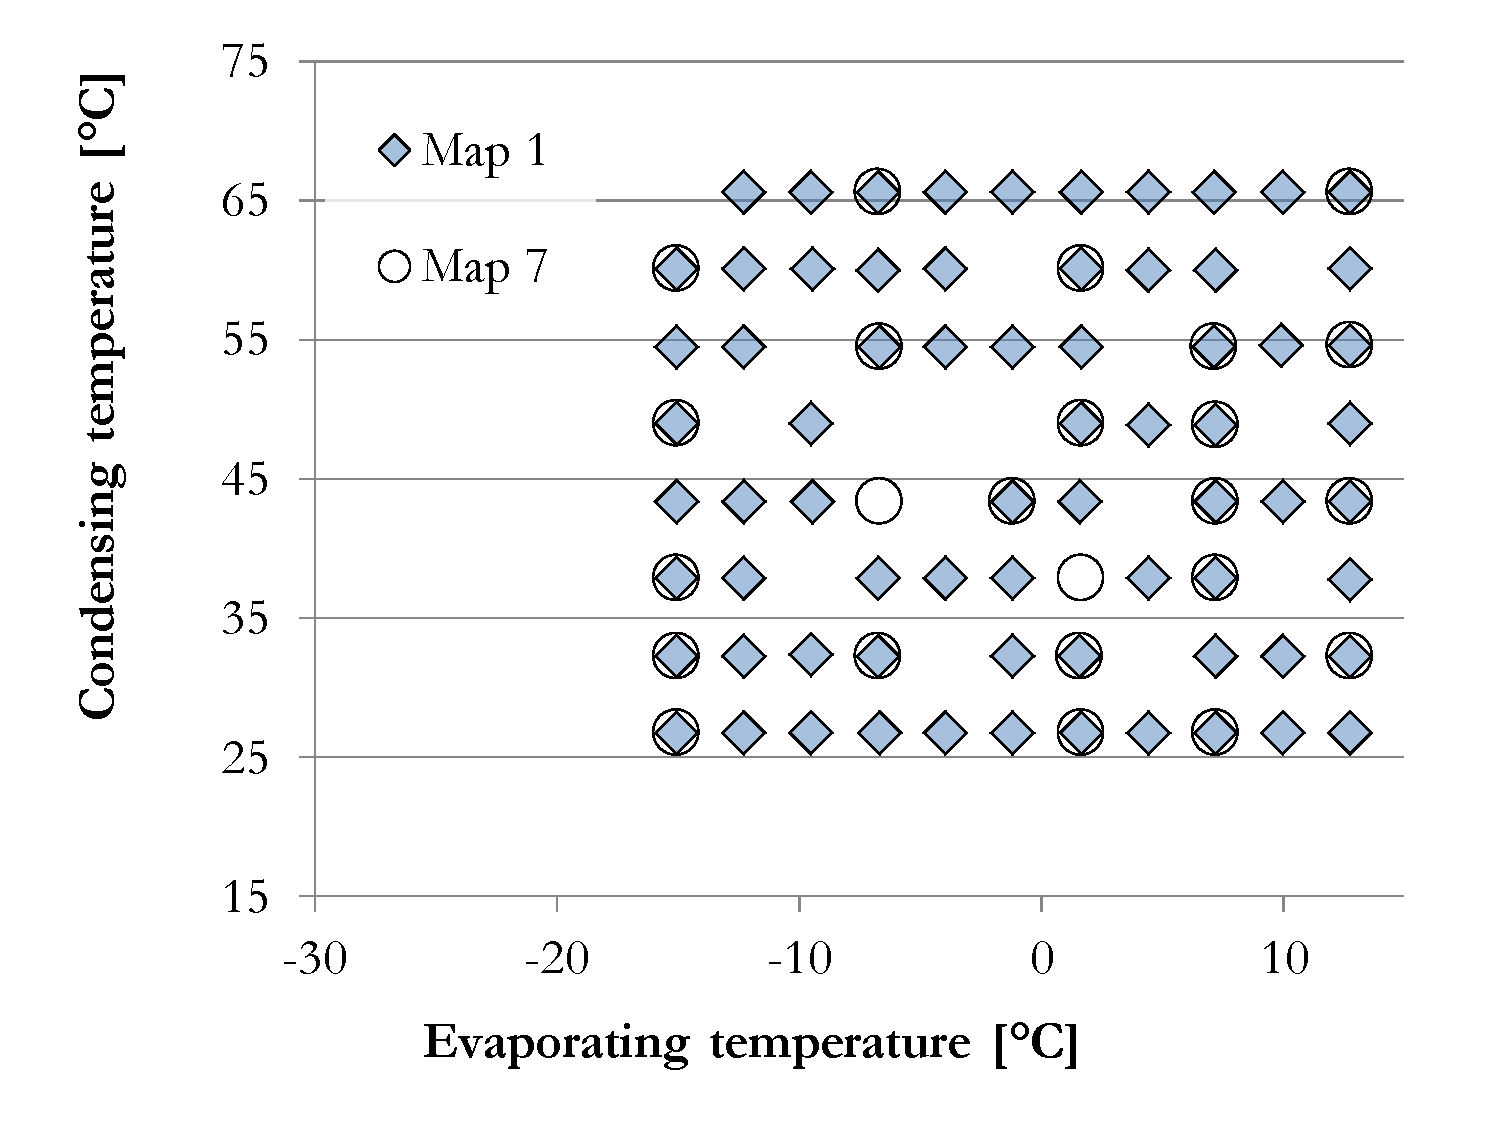
\includegraphics[width=15pc]{./fig/Map_1_and_7_training_data.pdf}
\caption{\label{fig:map_1_7_training_data}Training data points for Maps 1 and 7. Note the absence of low temperature training data.}
\end{minipage}\hspace{2pc}%
\begin{minipage}{15pc}
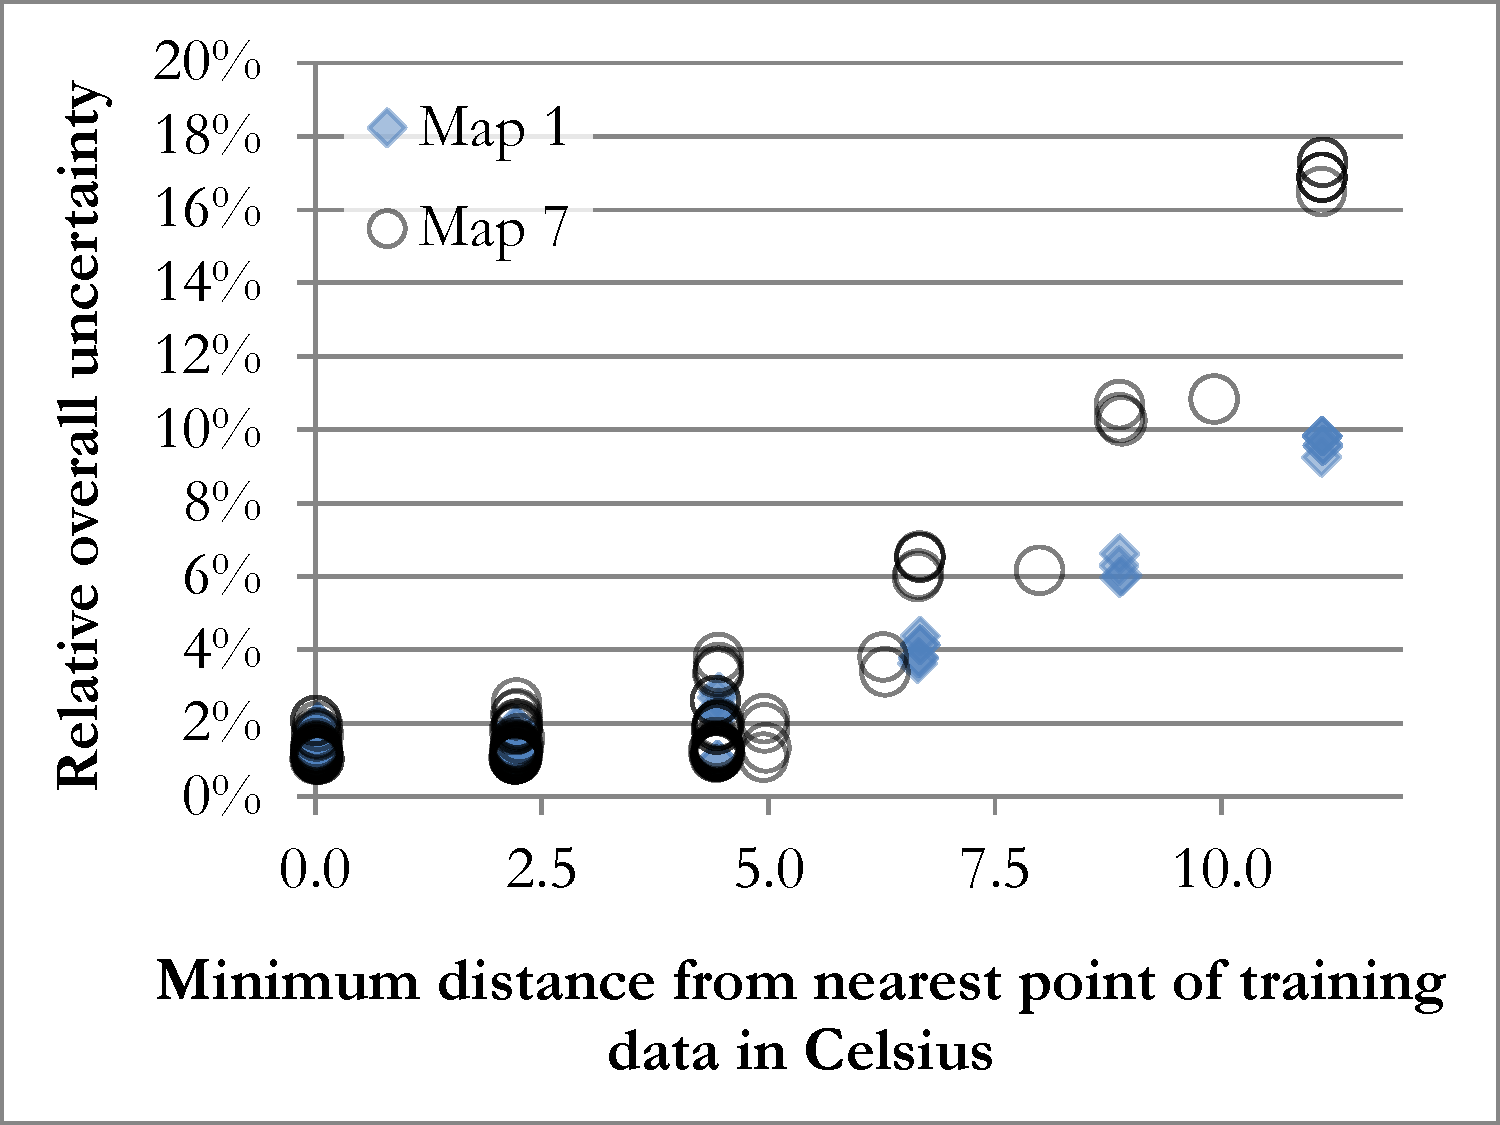
\includegraphics[width=15pc]{./fig/Map_1_and_7_C_distance.pdf}
\caption{\label{fig:map_1_7_unc_C_distance}Change of accuracy with distance to nearest training data point for maps 1 and 7.}
\end{minipage} 
\end{figure}





\blCom{conclusion}
\section{Conclusions} \label{sec:concl}

To conclude, this paper demonstrates how uncertainty of 10-coefficient compressor maps can be calculated based on the uncertainty due to inputs, the uncertainty due to model random error, the uncertainty due to training data and the uncertainty from outputs. It shows that a method to assess the acuracy and applicability of the map output without measured data outside the training data. It also shows that the range of training data and the number of training data points affect the accuracy and applicability of the map.

\blCom{Future work - NEED TO FINISH!}
\section{Future work}
\label{sec:future_work}
One of the basic assumptions in this paper is that individual measurement values are normally distributed around their average value. However, this might not be the case for actual measurement data. Therefore, experiments with actual compressor measurements should be conducted to check whether this assumption is appropriate.\\

\section*{References}
\bibliography{uncer_reference}

%\appendix
\section*{Appendix}
\setcounter{section}{1}
\begin{table}[h]
\caption{\label{tb:appendix}Training data}
\begin{center}
\begin{tabular}{llllllllll}
\br
$T_{cond}$ [$^\circ C$] &$T_{evap}$ [$^\circ C$] &$\dot{W}$ [W] &Map 1 & Map 2 & Map 3 & Map 4 & Map 5 & Map 6 & Map 7 \\
\mr
26.65$\pm$0.31 & -28.89$\pm$0.20 & 1672.3$\pm$10.1& & & & & $\surd$ & $\surd$ & \\
26.66$\pm$0.31 & -26.09$\pm$0.20 & 1756.2$\pm$10.5& & & & $\surd$ & $\surd$ & & \\
26.63$\pm$0.32 & -23.34$\pm$0.24 & 1845.0$\pm$12.0& & & $\surd$ & $\surd$ & $\surd$ & $\surd$ & \\
26.69$\pm$0.45 & -20.56$\pm$0.22 & 1917.3$\pm$12.1& & & $\surd$ & $\surd$ & $\surd$ & & \\
26.67$\pm$0.31 & -17.77$\pm$0.22 & 1987.9$\pm$13.1& & $\surd$ & $\surd$ & $\surd$ & $\surd$ & $\surd$ & \\
26.68$\pm$0.31 & -14.99$\pm$0.23 & 2051.7$\pm$13.2& $\surd$ & $\surd$ & $\surd$ & $\surd$ & $\surd$ & & $\surd$ \\
26.66$\pm$0.31 & -12.25$\pm$0.23 & 2119.0$\pm$14.0& $\surd$ & $\surd$ & $\surd$ & $\surd$ & $\surd$ & $\surd$ & \\
26.66$\pm$0.31 & -9.45$\pm$0.24 & 2185.3$\pm$13.9& $\surd$ & $\surd$ & $\surd$ & $\surd$ & $\surd$ & & \\
26.65$\pm$0.31 & -6.66$\pm$0.24 & 2249.1$\pm$14.1& $\surd$ & $\surd$ & $\surd$ & $\surd$ & $\surd$ & $\surd$ & \\
26.65$\pm$0.31 & -3.90$\pm$0.25 & 2320.3$\pm$14.7& $\surd$ & $\surd$ & $\surd$ & $\surd$ & $\surd$ & & \\
26.69$\pm$0.31 & -1.13$\pm$0.25 & 2397.2$\pm$16.2& $\surd$ & $\surd$ & $\surd$ & $\surd$ & $\surd$ & $\surd$ & \\
26.66$\pm$0.31 & 1.70$\pm$0.26 & 2466.9$\pm$16.3& $\surd$ & $\surd$ & $\surd$ & $\surd$ & $\surd$ & & $\surd$ \\
26.66$\pm$0.31 & 4.44$\pm$0.27 & 2536.8$\pm$17.1& $\surd$ & $\surd$ & $\surd$ & $\surd$ & $\surd$ & $\surd$ & \\
26.66$\pm$0.31 & 7.23$\pm$0.27 & 2624.8$\pm$16.8& $\surd$ & $\surd$ & $\surd$ & $\surd$ & $\surd$ & $\surd$ & $\surd$ \\
26.68$\pm$0.31 & 10.01$\pm$0.28 & 2717.1$\pm$17.6& $\surd$ & $\surd$ & & & & & \\
26.70$\pm$0.31 & 12.79$\pm$0.28 & 2808.1$\pm$18.6& $\surd$ & & & & & $\surd$ & \\
32.21$\pm$0.32 & -28.88$\pm$0.20 & 1686.0$\pm$10.7& & & & & $\surd$ & & \\
32.24$\pm$0.32 & -26.13$\pm$0.19 & 1817.7$\pm$12.2& & & & $\surd$ & $\surd$ & $\surd$ & \\
32.21$\pm$0.32 & -23.33$\pm$0.21 & 1950.9$\pm$12.4& & & $\surd$ & $\surd$ & $\surd$ & & \\
32.23$\pm$0.32 & -20.56$\pm$0.25 & 2072.8$\pm$13.8& & & $\surd$ & $\surd$ & $\surd$ & $\surd$ & \\
32.21$\pm$0.32 & -17.77$\pm$0.22 & 2192.6$\pm$14.2& & $\surd$ & $\surd$ & $\surd$ & $\surd$ & & \\
32.24$\pm$0.32 & -15.02$\pm$0.23 & 2305.9$\pm$14.7& $\surd$ & $\surd$ & $\surd$ & $\surd$ & $\surd$ & $\surd$ & $\surd$ \\
32.18$\pm$0.32 & -12.22$\pm$0.23 & 2407.7$\pm$16.0& $\surd$ & $\surd$ & $\surd$ & $\surd$ & $\surd$ & & \\
32.26$\pm$0.32 & -9.44$\pm$0.24 & 2530.9$\pm$15.4& $\surd$ & $\surd$ & $\surd$ & $\surd$ & $\surd$ & $\surd$ & \\
32.23$\pm$0.32 & -6.69$\pm$0.24 & 2653.7$\pm$17.4& $\surd$ & $\surd$ & $\surd$ & $\surd$ & $\surd$ & & $\surd$ \\
32.19$\pm$0.32 & -3.90$\pm$0.25 & 2749.0$\pm$17.9& & & $\surd$ & $\surd$ & $\surd$ & $\surd$ & \\
32.24$\pm$0.32 & -1.13$\pm$0.25 & 2853.2$\pm$20.3& $\surd$ & $\surd$ & $\surd$ & $\surd$ & $\surd$ & & \\
32.22$\pm$0.32 & 1.64$\pm$0.26 & 2982.5$\pm$18.3& $\surd$ & $\surd$ & $\surd$ & $\surd$ & $\surd$ & $\surd$ & $\surd$ \\
32.22$\pm$0.32 & 4.47$\pm$0.27 & 3099.6$\pm$20.3& & & $\surd$ & $\surd$ & $\surd$ & & \\
32.23$\pm$0.32 & 7.21$\pm$0.27 & 3223.1$\pm$20.9& $\surd$ & $\surd$ & $\surd$ & $\surd$ & $\surd$ & $\surd$ & \\
32.21$\pm$0.32 & 10.01$\pm$0.28 & 3357.7$\pm$21.8& $\surd$ & $\surd$ & & & & $\surd$ & \\
32.23$\pm$0.32 & 12.79$\pm$0.28 & 3484.5$\pm$22.0& $\surd$ & & & & & $\surd$ & $\surd$ \\
37.75$\pm$0.34 & -28.90$\pm$0.20 & 1598.1$\pm$11.2& & & & & $\surd$ & $\surd$ & \\
37.77$\pm$0.33 & -26.09$\pm$0.20 & 1782.5$\pm$11.3& & & & $\surd$ & $\surd$ & & \\
37.80$\pm$0.34 & -23.31$\pm$0.22 & 1949.3$\pm$12.0& & & $\surd$ & $\surd$ & $\surd$ & $\surd$ & \\
37.79$\pm$0.34 & -20.55$\pm$0.26 & 2114.0$\pm$13.4& & & $\surd$ & $\surd$ & $\surd$ & & \\
37.80$\pm$0.34 & -17.79$\pm$0.22 & 2281.3$\pm$14.5& & $\surd$ & & $\surd$ & $\surd$ & $\surd$ & \\
37.78$\pm$0.34 & -15.02$\pm$0.23 & 2436.0$\pm$14.5& $\surd$ & & $\surd$ & $\surd$ & $\surd$ & & $\surd$ \\
37.81$\pm$0.34 & -12.21$\pm$0.23 & 2588.4$\pm$16.4& $\surd$ & $\surd$ & & $\surd$ & & $\surd$ & \\
37.78$\pm$0.34 & -9.45$\pm$0.24 & 2742.2$\pm$17.1& & & $\surd$ & $\surd$ & & $\surd$ & \\
37.76$\pm$0.34 & -6.72$\pm$0.24 & 2892.5$\pm$19.4& $\surd$ & $\surd$ & & $\surd$ & $\surd$ & $\surd$ & \\
37.76$\pm$0.34 & -3.91$\pm$0.25 & 3049.7$\pm$19.8& $\surd$ & $\surd$ & $\surd$ & $\surd$ & $\surd$ & $\surd$ & \\
37.77$\pm$0.34 & -1.12$\pm$0.25 & 3194.3$\pm$20.0& $\surd$ & $\surd$ & & $\surd$ & $\surd$ & $\surd$ & \\
37.82$\pm$0.30 & 1.66$\pm$0.26 & 3364.8$\pm$21.8& & & $\surd$ & $\surd$ & $\surd$ & $\surd$ & $\surd$ \\
37.78$\pm$0.34 & 4.43$\pm$0.26 & 3512.7$\pm$22.5& $\surd$ & $\surd$ & $\surd$ & $\surd$ & $\surd$ & $\surd$ & \\
37.78$\pm$0.34 & 7.21$\pm$0.27 & 3665.8$\pm$24.2& $\surd$ & $\surd$ & $\surd$ & $\surd$ & $\surd$ & $\surd$ & $\surd$ \\
37.79$\pm$0.46 & 9.98$\pm$0.28 & 3830.4$\pm$25.5& & $\surd$ & & & & & \\
37.73$\pm$0.34 & 12.79$\pm$0.28 & 4002.3$\pm$25.6& $\surd$ & & & & & $\surd$ & \\
43.33$\pm$0.35 & -26.09$\pm$0.24 & 1660.6$\pm$10.2& & & & $\surd$ & $\surd$ & $\surd$ & \\
43.32$\pm$0.35 & -23.32$\pm$0.21 & 1883.8$\pm$11.8& & & $\surd$ & $\surd$ & $\surd$ & & \\
43.34$\pm$0.35 & -20.56$\pm$0.22 & 2088.4$\pm$13.6& & & $\surd$ & $\surd$ & $\surd$ & $\surd$ & \\
43.34$\pm$0.35 & -17.76$\pm$0.25 & 2287.1$\pm$14.6& & $\surd$ & $\surd$ & $\surd$ & $\surd$ & & \\
43.32$\pm$0.35 & -15.02$\pm$0.23 & 2490.0$\pm$15.9& $\surd$ & $\surd$ & $\surd$ & $\surd$ & $\surd$ & $\surd$ & \\
43.33$\pm$0.35 & -12.21$\pm$0.23 & 2679.1$\pm$18.2& $\surd$ & $\surd$ & $\surd$ & $\surd$ & $\surd$ & $\surd$ & \\
43.36$\pm$0.35 & -9.42$\pm$0.24 & 2872.1$\pm$17.8& $\surd$ & $\surd$ & $\surd$ & $\surd$ & & $\surd$ & \\
43.31$\pm$0.35 & -6.66$\pm$0.34 & 3064.2$\pm$19.5& & & & & & & $\surd$ \\
43.33$\pm$0.35 & -3.90$\pm$0.25 & 3240.6$\pm$21.7& & & & & & & \\
43.31$\pm$0.35 & -1.12$\pm$0.21 & 3434.6$\pm$21.1& $\surd$ & $\surd$ & $\surd$ & $\surd$ & $\surd$ & $\surd$ & $\surd$ \\
43.35$\pm$0.35 & 1.65$\pm$0.26 & 3610.0$\pm$23.0& $\surd$ & $\surd$ & $\surd$ & $\surd$ & $\surd$ & $\surd$ & \\
43.35$\pm$0.35 & 4.46$\pm$0.26 & 3793.5$\pm$24.8& & & $\surd$ & $\surd$ & $\surd$ & & \\
43.35$\pm$0.35 & 7.22$\pm$0.27 & 3990.4$\pm$24.4& $\surd$ & $\surd$ & $\surd$ & $\surd$ & $\surd$ & $\surd$ & $\surd$ \\
43.32$\pm$0.35 & 10.01$\pm$0.28 & 4193.4$\pm$25.9& $\surd$ & $\surd$ & & & & $\surd$ & \\
43.31$\pm$0.35 & 12.76$\pm$0.28 & 4394.6$\pm$27.0& $\surd$ & & & & & & $\surd$ \\
48.83$\pm$0.36 & -23.34$\pm$0.21 & 1776.1$\pm$11.9& & & $\surd$ & $\surd$ & $\surd$ & $\surd$ & \\
48.88$\pm$0.36 & -20.56$\pm$0.22 & 2015.6$\pm$12.7& & & $\surd$ & $\surd$ & $\surd$ & & \\
48.90$\pm$0.36 & -17.80$\pm$0.22 & 2262.8$\pm$14.8& & $\surd$ & & $\surd$ & $\surd$ & $\surd$ & \\
48.87$\pm$0.36 & -15.00$\pm$0.23 & 2489.0$\pm$15.7& $\surd$ & $\surd$ & $\surd$ & $\surd$ & $\surd$ & & $\surd$ \\
48.90$\pm$0.36 & -12.21$\pm$0.23 & 2718.8$\pm$18.3& & & & $\surd$ & $\surd$ & $\surd$ & \\
48.88$\pm$0.36 & -9.44$\pm$0.24 & 2933.5$\pm$18.9& $\surd$ & $\surd$ & $\surd$ & $\surd$ & $\surd$ & $\surd$ & \\
48.87$\pm$0.36 & -6.67$\pm$0.24 & 3150.8$\pm$20.1& & & & & & & \\
48.90$\pm$0.36 & -3.88$\pm$0.25 & 3377.9$\pm$21.1& & & & & & & \\
48.89$\pm$0.36 & -1.11$\pm$0.25 & 3587.6$\pm$23.2& & & & & & & \\
48.89$\pm$0.36 & 1.67$\pm$0.26 & 3804.8$\pm$25.0& $\surd$ & $\surd$ & $\surd$ & $\surd$ & $\surd$ & $\surd$ & $\surd$ \\
48.85$\pm$0.36 & 4.46$\pm$0.26 & 4029.1$\pm$24.1& $\surd$ & $\surd$ & $\surd$ & $\surd$ & $\surd$ & $\surd$ & \\
48.84$\pm$0.36 & 7.22$\pm$0.27 & 4232.9$\pm$26.0& $\surd$ & $\surd$ & $\surd$ & $\surd$ & $\surd$ & $\surd$ & $\surd$ \\
48.91$\pm$0.36 & 9.98$\pm$0.28 & 4457.1$\pm$29.4& & $\surd$ & & & & & \\
48.90$\pm$0.36 & 12.79$\pm$0.28 & 4702.3$\pm$32.1& $\surd$ & & & & & $\surd$ & \\
54.46$\pm$0.37 & -20.55$\pm$0.22 & 1961.8$\pm$12.1& & & $\surd$ & $\surd$ & $\surd$ & $\surd$ & \\
54.46$\pm$0.37 & -17.76$\pm$0.22 & 2231.4$\pm$14.1& & $\surd$ & $\surd$ & $\surd$ & $\surd$ & & \\
54.46$\pm$0.37 & -15.00$\pm$0.23 & 2484.4$\pm$17.0& $\surd$ & & $\surd$ & $\surd$ & $\surd$ & $\surd$ & \\
54.45$\pm$0.37 & -12.24$\pm$0.23 & 2750.2$\pm$17.7& $\surd$ & $\surd$ & $\surd$ & $\surd$ & $\surd$ & & \\
54.40$\pm$0.37 & -9.43$\pm$0.24 & 2996.3$\pm$19.0& & & $\surd$ & $\surd$ & $\surd$ & $\surd$ & \\
54.41$\pm$0.37 & -6.64$\pm$0.24 & 3257.1$\pm$22.8& $\surd$ & $\surd$ & $\surd$ & $\surd$ & $\surd$ & $\surd$ & $\surd$ \\
54.40$\pm$0.37 & -3.90$\pm$0.25 & 3486.9$\pm$23.1& $\surd$ & $\surd$ & $\surd$ & $\surd$ & $\surd$ & $\surd$ & \\
54.43$\pm$0.37 & -1.12$\pm$0.25 & 3720.8$\pm$25.1& $\surd$ & $\surd$ & $\surd$ & $\surd$ & $\surd$ & $\surd$ & \\
54.43$\pm$0.37 & 1.69$\pm$0.26 & 3973.5$\pm$25.2& $\surd$ & $\surd$ & $\surd$ & $\surd$ & $\surd$ & $\surd$ & \\
54.48$\pm$0.37 & 4.48$\pm$0.27 & 4219.8$\pm$24.9& & & $\surd$ & $\surd$ & $\surd$ & & \\
54.44$\pm$0.37 & 7.20$\pm$0.27 & 4463.8$\pm$27.9& $\surd$ & $\surd$ & $\surd$ & $\surd$ & $\surd$ & $\surd$ & $\surd$ \\
54.50$\pm$0.37 & 9.98$\pm$0.27 & 4704.9$\pm$32.2& $\surd$ & $\surd$ & & & & $\surd$ & \\
54.48$\pm$0.37 & 12.79$\pm$0.28 & 4959.9$\pm$30.5& $\surd$ & & & & & $\surd$ & $\surd$ \\
59.99$\pm$0.38 & -17.78$\pm$0.31 & 2215.3$\pm$14.3& & $\surd$ & $\surd$ & & & $\surd$ & \\
60.05$\pm$0.39 & -14.98$\pm$0.23 & 2509.3$\pm$16.5& $\surd$ & $\surd$ & $\surd$ & & & & $\surd$ \\
59.98$\pm$0.38 & -12.24$\pm$0.23 & 2800.7$\pm$18.2& $\surd$ & $\surd$ & $\surd$ & & & $\surd$ & \\
60.03$\pm$0.38 & -9.43$\pm$0.24 & 3073.9$\pm$19.8& $\surd$ & $\surd$ & $\surd$ & & & & \\
59.94$\pm$0.38 & -6.66$\pm$0.24 & 3343.6$\pm$22.0& $\surd$ & $\surd$ & $\surd$ & & & $\surd$ & \\
60.00$\pm$0.38 & -3.91$\pm$0.25 & 3612.7$\pm$23.0& $\surd$ & $\surd$ & $\surd$ & & & & \\
60.03$\pm$0.38 & -1.11$\pm$0.12 & 3874.9$\pm$27.1& & & $\surd$ & & & $\surd$ & \\
60.03$\pm$0.38 & 1.68$\pm$0.26 & 4143.5$\pm$26.4& $\surd$ & $\surd$ & $\surd$ & & & & $\surd$ \\
59.97$\pm$0.38 & 4.45$\pm$0.27 & 4402.2$\pm$26.5& $\surd$ & $\surd$ & $\surd$ & & & $\surd$ & \\
59.96$\pm$0.38 & 7.23$\pm$0.27 & 4669.3$\pm$29.6& $\surd$ & $\surd$ & $\surd$ & & & & \\
60.04$\pm$0.38 & 9.98$\pm$0.28 & 4943.1$\pm$32.4& & $\surd$ & & & & $\surd$ & \\
60.02$\pm$0.38 & 12.81$\pm$0.28 & 5197.5$\pm$35.6& $\surd$ & & & & & & \\
65.55$\pm$0.40 & -12.21$\pm$0.23 & 2918.1$\pm$18.8& $\surd$ & $\surd$ & & & & $\surd$ & \\
65.53$\pm$0.40 & -9.49$\pm$0.24 & 3210.6$\pm$20.8& $\surd$ & $\surd$ & & & & & \\
65.57$\pm$0.39 & -6.68$\pm$0.24 & 3495.6$\pm$22.5& $\surd$ & $\surd$ & & & & $\surd$ & $\surd$ \\
65.51$\pm$0.40 & -3.89$\pm$0.25 & 3792.3$\pm$24.8& $\surd$ & $\surd$ & & & & $\surd$ & \\
65.58$\pm$0.40 & -1.11$\pm$0.25 & 4066.9$\pm$24.7& $\surd$ & $\surd$ & & & & & \\
65.54$\pm$0.40 & 1.67$\pm$0.26 & 4348.6$\pm$28.5& $\surd$ & $\surd$ & & & & $\surd$ & \\
65.56$\pm$0.40 & 4.44$\pm$0.26 & 4626.5$\pm$28.9& $\surd$ & $\surd$ & & & & $\surd$ & \\
65.57$\pm$0.40 & 7.20$\pm$0.27 & 4927.9$\pm$31.3& $\surd$ & $\surd$ & & & & & \\
65.56$\pm$0.40 & 10.02$\pm$0.28 & 5206.3$\pm$33.6& $\surd$ & $\surd$ & & & & $\surd$ & \\
65.55$\pm$0.39 & 12.77$\pm$0.28 & 5478.7$\pm$34.5& $\surd$ & & & & & $\surd$ & $\surd$ \\
\br
\end{tabular}
\end{center}
\end{table}


\end{document}


